%File: main.tex -- AI6103 group project report, AAAI-24 camera-ready template
\documentclass[letterpaper]{article} % DO NOT CHANGE THIS
\usepackage{aaai24}  % DO NOT CHANGE THIS
\usepackage{times}  % DO NOT CHANGE THIS
\usepackage{helvet}  % DO NOT CHANGE THIS
\usepackage{courier}  % DO NOT CHANGE THIS
\usepackage[hyphens]{url}  % DO NOT CHANGE THIS
\usepackage{graphicx} % DO NOT CHANGE THIS
\urlstyle{rm} % DO NOT CHANGE THIS
\def\UrlFont{\rm}  % DO NOT CHANGE THIS
\usepackage{natbib}  % DO NOT CHANGE THIS AND DO NOT ADD ANY OPTIONS TO IT
\usepackage{caption} % DO NOT CHANGE THIS AND DO NOT ADD ANY OPTIONS TO IT
\frenchspacing  % DO NOT CHANGE THIS
\setlength{\pdfpagewidth}{8.5in}  % DO NOT CHANGE THIS
\setlength{\pdfpageheight}{11in}  % DO NOT CHANGE THIS

\usepackage{amsmath}
\usepackage{amssymb}
\usepackage{booktabs}

\pdfinfo{
/TemplateVersion (2024.1)
}

% This is a course report, not an AAAI publication, so the AAAI copyright notice is switched off.
\nocopyright

\setcounter{secnumdepth}{2}

\newcommand{\E}{\mathbb{E}}
\newcommand{\Sg}{\Sigma_g}
\newcommand{\norm}[1]{\lVert #1\rVert}
\newcommand{\Tr}{\operatorname{Tr}}
\newcommand{\sig}{$^{*}$}

\title{Does the Gradient Matter? Gradient-Weighted Explained Variance Adaptation for LoRA Initialisation}
\author{
    {[Name]} ([Matric No.]),
    {[Name]} ([Matric No.]),
    {[Name]} ([Matric No.]),\\
    {[Name]} ([Matric No.]),
    {[Name]} ([Matric No.]),
    Yin Chenyu ([Matric No.])
}
\affiliations{
    AI6103 Deep Learning, Group Project (Option 2: improve on an existing codebase)\\
    College of Computing and Data Science, Nanyang Technological University, Singapore\\
    {[email]}@e.ntu.edu.sg, {[email]}@e.ntu.edu.sg, {[email]}@e.ntu.edu.sg,\\
    {[email]}@e.ntu.edu.sg, {[email]}@e.ntu.edu.sg, {[email]}@e.ntu.edu.sg\\
    Code and all run files: \url{https://github.com/Xander-YangXH/NTU-AI6103-DL-Project}
}

\begin{document}

\maketitle

\begin{abstract}
EVA initialises LoRA's down-projection $A$ with the principal components of each layer's input activations. Its optimality argument assumes that the gradient arriving at a layer's output is independent of that layer's input. We drop this assumption and show that, at initialisation, the expected squared per-token gradient on $B$ is exactly $\Tr(A\Sg A^\top)$ with $\Sg=\E[\norm{g}^2xx^\top]$. Its maximiser, the top eigenspace of $\Sg$, defines GW-EVA, and a mini-batch version of the same identity places EVA, GW-EVA and LoRA-GA in one family. We implement GW-EVA on Hugging Face PEFT and compare nine initialisations on RoBERTa-base under one protocol: GLUE SST-2, MRPC and RTE, plus a 1,000-example SST-2 subset, with seed-paired statistics over about 300 fine-tuning runs. The theory holds. A magnitude-only control raises the step-0 gradient by the predicted factor $\sqrt{3}$ (measured 1.78--1.83), GW-EVA raises it a further 1.5--2.3$\times$ over EVA, and GW-EVA's top-8 subspace overlaps EVA's only 0.49--0.69, against 0.84--0.95 between two independent GW-EVA estimates. None of this reaches the final accuracy. GW-EVA $-$ EVA is $-0.15$, $-0.88$, $-1.23$ and $-0.46$ points on the four settings, and every 95\% interval contains 0. No initialisation beats plain LoRA at a tuned learning rate. EVA's 2.6-point deficit in low resource shrinks to an insignificant 0.6 points at a lower learning rate, and calibrating EVA on generic text or another task moves 30--50\% of its subspace without changing accuracy. At rank 8 on RoBERTa-base, the directions $A$ starts from have little effect on final accuracy: larger initial gradients and faster early fitting are real but transient.
\end{abstract}

%=====================================================================
\section{Introduction}

LoRA \citep{hu2022lora} fine-tunes a frozen weight $W$ by adding a low-rank product $BA$, with $B=0$ and $A$ random at the start. A line of recent work replaces the random $A$ with a data-driven one. EVA \citep{paischer2025eva} takes the top right-singular vectors of each layer's input activations and redistributes ranks across layers by explained variance. LoRA-GA \citep{wang2024loraga} takes the singular vectors of the full-batch gradient, and PiSSA \citep{meng2024pissa} the principal components of $W$ itself. These methods report faster convergence and higher accuracy, and are usually motivated by how much gradient signal the adapter receives at step 0.

EVA's optimality result rests on an assumption that is easy to miss: the output gradient $g=\partial L/\partial y$ is statistically independent of the input $x$. Our starting point is to remove this assumption. Doing so gives a closed-form objective whose maximiser is a gradient-weighted covariance. It also shows how EVA and LoRA-GA are two ends of the same objective. Our contributions are:

\begin{enumerate}
\item \textbf{Identity and new initialisation.} An exact identity for the expected step-0 gradient on $B$ without the independence assumption, and the resulting initialisation GW-EVA (Section~\ref{sec:method}). A mini-batch decomposition shows that EVA, GW-EVA and LoRA-GA maximise different terms of the same quantity.
\item \textbf{Implementation.} GW-EVA on PEFT \citep{mangrulkar2022peft}, with a per-token gradient hook, plus a parameter-cost rank allocation as a controlled factor.
\item \textbf{Controlled comparison.} Nine initialisations under one protocol, with matched parameter budgets, shared data splits, shared seeds and same-seed paired confidence intervals. The design includes a magnitude-only control (G2), which separates the effect of $A$'s direction from its norm, and two calibration-source controls (G8, G9).
\item \textbf{A negative result with its mechanism.} The theory holds, the larger gradients are real, and GW-EVA's subspace is measurably different from EVA's, yet none of this translates into accuracy. The apparent wins of data-aware initialisations disappear once learning rate and GPU are controlled.
\end{enumerate}

%=====================================================================
\section{Background and Related Work}

\subsection{LoRA}
For a frozen weight $W\in\mathbb{R}^{d_{out}\times d_{in}}$ and input $x$, LoRA computes $y=Wx+\frac{\alpha}{r}BAx$ with $A\in\mathbb{R}^{r\times d_{in}}$ and $B\in\mathbb{R}^{d_{out}\times r}$. Only $A$ and $B$ are trained. $B$ starts at zero, so the adapted model initially equals the pre-trained one. PEFT initialises $A$ with Kaiming-uniform noise $U(\pm 1/\sqrt{d_{in}})$ \citep{he2015delving}.

\subsection{EVA}
\label{sec:eva}
EVA \citep{paischer2025eva} sets $A$ in two steps, before fine-tuning starts.

\textbf{Directions by incremental SVD.} Mini-batches of calibration data are passed through the frozen model. For every adapted layer, the inputs $x$ of all non-padding tokens are collected and an incremental truncated SVD \citep{ross2008incremental} of this activation matrix is updated after each batch, keeping $\rho r$ components. A component counts as converged when the cosine similarity between its estimates after two consecutive batches reaches $\tau$ (0.99 here), and calibration stops once every layer has converged.

\textbf{Ranks by explained variance.} Each component $j$ of layer $i$ gets an explained-variance ratio $\xi^i_j=(\sigma^i_j)^2/\big((M-1)\norm{\sigma^i}_1\big)$, where $\sigma^i$ are the layer's singular values and $M$ is the number of samples seen. All components of all layers are sorted by $\xi$, and the top $N r$ are kept for $N$ adapted layers. A layer's rank is the number of its components in that selection, at most $\rho r$. The kept right-singular vectors, which are unit rows, become $A$, and $B=0$. PEFT rescales $\alpha$ with the new rank so that $\alpha/r$ is unchanged.

EVA's Theorem~3.2 states that this choice maximises the expected squared gradient on $B$, $\E\norm{\partial L/\partial B}_F^2\propto\Tr(A\Sigma A^\top)$ with $\Sigma=\E[xx^\top]$. The proportionality holds only if the output gradient is independent of the input; the paper's NTK argument makes the same assumption explicitly. PEFT's implementation centres the activations, so in practice EVA uses the principal components of the centred activation covariance.

\subsection{Other Initialisations and Rank Allocation}
Data-driven initialisations differ in which statistic they use (Table~\ref{tab:methods}). LoRA-GA also sets $B\neq 0$ and subtracts $BA$ from $W$ to keep the initial function unchanged. GW-EVA sits between EVA and LoRA-GA: it uses activations weighted by per-token gradient norms, but not the gradient's direction.

\begin{table}[t]
\centering
\small
\begin{tabular}{@{}p{0.27\columnwidth}p{0.48\columnwidth}l@{}}
\toprule
Method & Statistic used & Labels \\
\midrule
PiSSA & Principal components of $W$ & No \\
EVA & Principal components of the layer inputs & No \\
LoRA-GA & Singular vectors of the mean gradient $\partial L/\partial W$ & Yes \\
GW-EVA (ours) & Principal components of the inputs, weighted by per-token gradient norms & Yes \\
\bottomrule
\end{tabular}
\caption{Statistics used by data-driven LoRA initialisations.}
\label{tab:methods}
\end{table}

AdaLoRA \citep{zhang2023adalora} prunes ranks during training by an importance score, while EVA allocates ranks once, before training, at a fixed total rank count. A fixed rank count is not a fixed parameter count: a rank in a 768$\to$3072 FFN layer costs 2.5$\times$ as many parameters as one in a 768$\to$768 attention projection. We therefore also test an allocation that ranks components by explained variance per parameter (Section~\ref{sec:cost}).

%=====================================================================
\section{Method}
\label{sec:method}

\subsection{Setting}
Consider one adapted linear layer $y=Wx+\frac{\alpha}{r}BAx$ with $\alpha=r$. For one token, write $g=\partial L/\partial y$. At initialisation $B=0$, so the layer output, and hence $g$, does not depend on $A$.

\subsection{The Step-0 Gradient on $B$}
\label{sec:identity}
For one token, $\partial L/\partial B=g\,(Ax)^\top$, so $\norm{\partial L/\partial B}_F^2=\norm{g}^2\norm{Ax}^2=\norm{g}^2x^\top A^\top Ax$. Taking expectations over tokens,
\begin{equation}
\E\Big\lVert\frac{\partial L}{\partial B}\Big\rVert_F^2=\Tr\big(A\Sg A^\top\big),\qquad \Sg=\E\big[\norm{g}^2xx^\top\big].
\label{eq:identity}
\end{equation}
This is exact. Because $g$ does not depend on $A$ at $B=0$, $\Sg$ is the same matrix for every candidate $A$. By Ky Fan's theorem \citep{fan1949theorem}, the maximiser over $A$ with orthonormal rows is the top-$r$ eigenvectors of $\Sg$.

\textbf{EVA as a special case.} If $\norm{g}^2$ is independent of $x$, then $\Sg=\E\norm{g}^2\cdot\E[xx^\top]$, whose eigenvectors are those of the uncentred activation second moment. EVA computes the centred version (Section~\ref{sec:eva}); the two coincide when the activations have zero mean. EVA is therefore optimal for this objective only when the per-token gradient magnitude carries no information about the input.

\textbf{Magnitude.} If $A$'s directions are independent of $\Sg$, the expected gradient scales with $A$'s squared row norm. Kaiming-uniform rows have $\E\norm{a}^2=d_{in}\cdot\frac{1}{3d_{in}}=\frac{1}{3}$, while orthonormal rows have norm 1. A random orthonormal $A$ (our G2) should therefore give a step-0 gradient norm $\sqrt{3}\approx1.73$ times that of LoRA (G1). This is a falsifiable check of the identity (Section~\ref{sec:step0}).

\subsection{Mini-Batch View: EVA, GW-EVA and LoRA-GA}
The optimiser sees the mean gradient over a batch of $m$ tokens, $\bar G_m=\frac{1}{m}\sum_i g_ix_i^\top$. If the $m$ tokens are drawn independently, expanding the square gives
\begin{equation}
\E\norm{\bar G_mA^\top}_F^2=\tfrac{1}{m}\Tr\big(A\Sg A^\top\big)+\big(1-\tfrac{1}{m}\big)\norm{\E[gx^\top]A^\top}_F^2 .
\label{eq:minibatch}
\end{equation}
The first term is the per-token objective above, maximised by GW-EVA, and by EVA under independence. The second term is maximised by the top right-singular vectors of the expected gradient $\E[gx^\top]$, which is LoRA-GA's choice. The three methods are therefore solutions of one objective under different assumptions about the batch size and about the dependence between $g$ and $x$.

\subsection{GW-EVA}
For each of the 72 adapted layers, GW-EVA proceeds as follows.
\begin{enumerate}
\item \textbf{Warm up the head.} Train the classification head for one epoch with the encoder frozen, as every group does. Without this, $g$ would reflect a random head.
\item \textbf{Calibrate.} Run 1,024 labelled training examples, in batches of 16, through the model. A forward hook stores each token's input $x$ and a backward hook stores $\norm{g}$ at the layer output. Padding tokens are masked.
\item \textbf{Sketch $\Sg$.} Accumulate the weighted inputs $x\norm{g}$ in a streaming truncated SVD, without centring, so that the sketch estimates the uncentred second moment $\Sg$.
\item \textbf{Set $A$.} Take the top components as $A$'s rows. Allocate ranks as EVA does: compute up to $\rho r=16$ components per layer and keep the globally highest explained-variance ratios, at a total of 576 ranks.
\item \textbf{Keep the starting function.} Set $B=0$ and leave $W$ unchanged.
\end{enumerate}
The extra cost over EVA is one backward pass per calibration batch.

\subsection{Parameter-Cost Allocation}
\label{sec:cost}
With a total of 576 ranks, EVA's allocation can over- or under-spend the parameter budget of uniform $r=8$, which is 1,327,104 for RoBERTa-base. Our alternative scores every candidate component by its explained-variance ratio divided by its parameter cost $d_{in}+d_{out}$ (1,536 for an attention projection, 3,840 for an FFN layer). It then fills the budget greedily, skipping components that no longer fit, with at most 16 ranks per layer. Because all components of a layer cost the same, each layer always receives a prefix of its components. This solves
\begin{align}
&\max_{r_\ell}\ \sum_\ell\sum_{i\le r_\ell}\xi_{\ell,i}\nonumber\\
&\text{s.t.}\ \sum_\ell r_\ell\,(d_{in}+d_{out})\le 1{,}327{,}104,\quad 0\le r_\ell\le 16 .
\end{align}
G4 applies it to EVA's components and G6 to GW-EVA's. Every G4 and G6 allocation lands within 0.1\% of the budget.

\subsection{Controls}
\label{sec:controls}
\textbf{G2 (magnitude control).} $A$ has $r$ random orthonormal rows, from the QR decomposition of a Gaussian matrix, so each row has norm 1 like EVA's. The adapter is first built exactly as for G1 and $A$ is then overwritten from an independent generator, so for each seed G1 and G2 share the head, the warm-up, the batch order and every other random draw. Only $A$ differs.

\textbf{G7 (LoRA-GA).} After the head warm-up, the mean gradient $G$ of each adapted weight is estimated on 1,024 labelled training examples. With $G=USV^\top$, the authors' ArB2r scheme sets $A=c\,V_{:,1:r}^\top$ and $B=c\,U_{:,r+1:2r}$ with $c=d_{out}^{1/4}/\sqrt{16}$, and replaces $W$ by $W-\frac{\alpha}{r}BA$ so that the initial function is unchanged. $A$ and $B$ are both non-zero and trainable from the first step.

\textbf{G8 (generic calibration).} G8 takes exactly G3's 1,024 calibration examples and keeps each example's token layout: total length, single-sentence or sentence-pair format, segment lengths and special-token positions. Only the tokens inside each segment are replaced by contiguous wikitext-103 text \citep{merity2017pointer}, so G3 and G8 differ only in content.

\textbf{G9 (cross-task calibration).} G9 calibrates EVA on another task's training data: SST-2 from MRPC, MRPC from RTE, and RTE from MRPC.

%=====================================================================
\section{Experimental Design}

\subsection{Groups and Hypotheses}
The core is a $2\times2$ factorial design, direction $\times$ allocation (G3--G6), plus five reference groups (Table~\ref{tab:groups}). We test four hypotheses.
\begin{itemize}
\item \textbf{H1.} In RoBERTa-base, $\norm{g}^2$ is correlated with $x$, and the top-$r$ subspaces of $\Sg$ and of the activation covariance differ measurably.
\item \textbf{H2.} At equal parameter count, GW-EVA has a larger step-0 gradient, a lower loss over the first 500 steps, and higher accuracy than EVA.
\item \textbf{H3.} Allocating ranks by parameter cost changes the result under a fixed budget.
\item \textbf{H4.} EVA's activation subspace is task-specific: calibrating on generic text or another task changes both the subspace and the accuracy.
\end{itemize}

\begin{table}[t]
\centering
\small
\setlength{\tabcolsep}{4pt}
\begin{tabular}{@{}p{0.17\columnwidth}p{0.30\columnwidth}p{0.17\columnwidth}p{0.22\columnwidth}@{}}
\toprule
Group & Direction of $A$ & Allocation & Tests \\
\midrule
G1 LoRA & Kaiming-uniform random & Uniform & Baseline \\
G2 & Random orthonormal, row norm 1 & Uniform & Magnitude \\
G3 EVA & Activation covariance & Rank count & Reproduction \\
G4 & Activation covariance & Param.\ cost & H3 \\
G5 GW-EVA & $\Sg$ & Rank count & H2 \\
G6 & $\Sg$ & Param.\ cost & H2, H3 \\
G7 LoRA-GA & Mean-gradient SVD; $B\neq0$, $W$ compensated & Uniform & 2nd term of Eq.~\ref{eq:minibatch} \\
G8 & Activation cov.\ on wikitext-103 & Rank count & H4 \\
G9 & Activation cov.\ on another task & Rank count & H4 \\
\bottomrule
\end{tabular}
\caption{Experimental groups. Uniform allocation is $r=8$ in every layer; rank-count allocation is EVA's ($\rho=2$).}
\label{tab:groups}
\end{table}

\subsection{Shared Protocol}
All groups follow the protocol in Table~\ref{tab:protocol}. Each group tunes its own learning rate on the same grid, including the LoRA baseline, so no group is handicapped by another's choice. Table~\ref{tab:lr} lists the chosen rates.

\begin{table}[t]
\centering
\small
\begin{tabular}{@{}p{0.22\columnwidth}p{0.72\columnwidth}@{}}
\toprule
Setting & Value \\
\midrule
Model, tasks & RoBERTa-base \citep{liu2019roberta}; GLUE SST-2, MRPC, RTE \citep{wang2019glue}; a 1,000-example SST-2 subset (seed 2027) \\
Adapters & All 72 attention ($q,k,v,o$) and FFN linear layers; $r=8$, $\alpha/r=1$, dropout 0; budget 1,327,104 parameters \\
Data split & 10\% of each training set held out as dev (seed 2026); final runs train on the other 90\% \\
Training & AdamW \citep{kingma2015adam,loshchilov2019decoupled}, batch 32, max length 128, linear schedule with 6\% warm-up, weight decay 0, bf16, no gradient clipping \\
Epochs & SST-2 3, MRPC 10, RTE 10, low resource 20 \\
Head warm-up & 1 epoch at lr $10^{-3}$, encoder frozen \\
Learning rate & Per group and task from $\{2,5,10\}\times10^{-4}$ on dev, seed 0; low resource reuses the full-SST-2 choice; G8/G9 reuse G3's \\
Calibration & 1,024 training examples, batch 16; $\tau=0.99$, $\rho=2$ \\
Seeds & SST-2 0--2; MRPC, RTE, low resource 0--4 (G5/G6 low resource 0--2) \\
Evaluation & Last epoch on the official validation set (accuracy; F1 for MRPC); never used for selection \\
\bottomrule
\end{tabular}
\caption{Shared protocol.}
\label{tab:protocol}
\end{table}

\begin{table}[t]
\centering
\small
\setlength{\tabcolsep}{3.5pt}
\begin{tabular}{@{}lcccccccc@{}}
\toprule
Task & G1 & G2 & G3 & G4 & G5 & G6 & G7 & G8/G9 \\
\midrule
SST-2 & 5e-4 & 5e-4 & 1e-3 & 5e-4 & 1e-3 & 5e-4 & 2e-4 & 1e-3 \\
MRPC & 2e-4 & 1e-3 & 2e-4 & 2e-4 & 2e-4 & 2e-4 & 2e-4 & 2e-4 \\
RTE & 5e-4 & 2e-4 & 2e-4 & 2e-4 & 2e-4 & 2e-4 & 2e-4 & 2e-4 \\
Low res. & 5e-4 & -- & 1e-3 & -- & 1e-3 & 5e-4 & -- & 1e-3 (G8) \\
\bottomrule
\end{tabular}
\caption{Learning rates chosen on the dev split.}
\label{tab:lr}
\end{table}

\subsection{Statistics}
All groups share the data split, the head warm-up and the seeds, and G1--G4 and G8 also share the batch order, so runs with the same seed are paired. We report the mean paired difference with a $t$-based 95\% interval (df $=n-1$) and mark intervals that exclude 0 with $^{*}$. Each table contains about 20 comparisons and is not corrected for multiplicity. Subspaces are compared by the mean squared cosine of the principal angles between the row spaces of two $A$ matrices, $\norm{Q_a^\top Q_b}_F^2/\min(k_a,k_b)$, averaged over the 72 layers. It is 1 for identical subspaces and about $r/d\approx0.01$ for random ones.

\subsection{Runs, Compute and Reproduction}
Under the shared protocol we ran 201 fine-tuning runs: 18 tuning runs each for G1/G2, G3/G4 and G5/G6 and 9 for G7; 26 main runs each for G1/G2, G3/G4 and G5/G6 and 13 each for G7, G8 and G9; and 5, 5, 6 and 5 low-resource runs for G1/G2, G3/G4, G5/G6 and G8. A further 95 runs hold the controls and extra seeds (40 extra seeds for G1 and G3; 55 learning-rate, $\rho$ and same-GPU controls), all on L40S. The H1 diagnosis adds 12 calibration-only runs. One run takes about 1--4 minutes on MRPC or RTE and 3--8 minutes on SST-2 on one GPU, mostly on the NTU CCDS TC2 cluster. G1/G2, G7, G8 and all controls ran on NVIDIA L40S, G3/G4 on A40 and G9 on an RTX 3050 Ti laptop GPU; G5/G6 did not record their GPU. All groups used torch 2.11, transformers 5.21 (G9: 5.20) and PEFT 0.21.2, except G7 (torch 2.4.0, transformers 4.52.4, PEFT 0.17.1). Every run writes one JSON file; \texttt{summary/collect.py} rebuilds all tables from them and \texttt{summary/figures.py} the figures.


%=====================================================================
\section{Results}

\subsection{Main Results}

\begin{table*}[t]
\centering
\small
\setlength{\tabcolsep}{2.5pt}
\begin{tabular}{@{}lccccccccc@{}}
\toprule
Task & G1 & G2 & G3 & G4 & G5 & G6 & G7 & G8 & G9 \\
\midrule
SST-2 (acc) & 93.92$\pm$0.00$^{\dagger}$ & 94.07$\pm$0.24 & 94.19$\pm$0.43 & 93.65$\pm$0.24 & 94.04$\pm$0.30 & \textbf{94.30$\pm$0.24} & 93.96$\pm$0.46 & 93.88$\pm$0.46 & 94.00$\pm$0.63 \\
MRPC (F1) & 91.34$\pm$0.43 & 91.16$\pm$1.11 & \textbf{92.02$\pm$0.79} & 91.50$\pm$0.68 & 91.14$\pm$0.69 & 91.41$\pm$0.52 & 91.83$\pm$0.46 & 91.11$\pm$0.34 & 91.50$\pm$0.60 \\
RTE (acc) & 73.94$\pm$2.10 & 73.86$\pm$1.04 & 74.80$\pm$2.49 & 73.57$\pm$2.06 & 73.57$\pm$2.43 & 72.92$\pm$2.09 & 56.68$\pm$8.85 & 72.06$\pm$2.18 & \textbf{75.67$\pm$1.70} \\
Low-res.\ SST-2 & \textbf{91.44$\pm$0.28} & -- & 88.81$\pm$0.83 & -- & 88.46$\pm$0.29 & 89.98$\pm$0.18 & -- & 89.89$\pm$0.52 & -- \\
\bottomrule
\end{tabular}
\caption{Official validation, mean $\pm$ sd (\%). $^{\dagger}$All three G1 seeds end with 819 of 872 examples correct; their training losses and per-epoch accuracies differ, so the zero standard deviation is a coincidence, not a repeated run.}
\label{tab:main}
\vspace{0.8em}
\setlength{\tabcolsep}{4pt}
\begin{tabular}{@{}lcccc@{}}
\toprule
Comparison & SST-2 & MRPC & RTE & Low resource \\
\midrule
G3 $-$ G1 (EVA vs LoRA) & $+0.27$ [$-0.81$, $+1.35$] & $+0.68$ [$-0.60$, $+1.97$] & $+0.87$ [$-3.27$, $+5.01$] & $-2.64$ [$-3.70$, $-1.57$]$^{*}$ \\
G5 $-$ G1 (GW-EVA vs LoRA) & $+0.11$ [$-0.64$, $+0.87$] & $-0.20$ [$-1.14$, $+0.75$] & $-0.36$ [$-5.35$, $+4.63$] & $-3.10$ [$-3.59$, $-2.60$]$^{*}$ \\
G7 $-$ G1 (LoRA-GA vs LoRA) & $+0.04$ [$-1.11$, $+1.19$] & $+0.49$ [$-0.44$, $+1.41$] & $-17.26$ [$-27.93$, $-6.59$]$^{*}$ & -- \\
\textbf{G5 $-$ G3 (H2)} & $-0.15$ [$-1.07$, $+0.76$] & $-0.88$ [$-2.05$, $+0.29$] & $-1.23$ [$-4.09$, $+1.64$] & $-0.46$ [$-3.82$, $+2.90$] \\
G4 $-$ G3 (H3, EVA) & $-0.54$ [$-1.69$, $+0.62$] & $-0.52$ [$-1.56$, $+0.52$] & $-1.23$ [$-4.31$, $+1.85$] & -- \\
G6 $-$ G5 (H3, GW-EVA) & $+0.27$ [$-0.65$, $+1.18$] & $+0.27$ [$-0.75$, $+1.28$] & $-0.65$ [$-6.19$, $+4.89$] & $+1.53$ [$+0.94$, $+2.12$]$^{*}$ \\
G8 $-$ G3 (H4, generic text) & $-0.31$ [$-2.31$, $+1.70$] & $-0.91$ [$-1.54$, $-0.28$]$^{*}$ & $-2.74$ [$-6.65$, $+1.16$] & $+1.08$ [$-0.09$, $+2.24$] \\
G9 $-$ G3 (H4, another task) & $-0.19$ [$-1.63$, $+1.24$] & $-0.52$ [$-1.21$, $+0.17$] & $+0.87$ [$-3.31$, $+5.04$] & -- \\
\bottomrule
\end{tabular}
\caption{Paired differences (points, 95\% CI; $^{*}$ = interval excludes 0).}
\label{tab:paired}
\end{table*}

Tables~\ref{tab:main} and~\ref{tab:paired} give the main results. On the three full-data tasks, every group except G7 lies within $\pm$1.9 points of LoRA, and every interval against G1 contains 0. The best and worst of G2--G6, G8 and G9 differ by less than 1 point on SST-2 and MRPC, and by less than the seed noise on RTE.

\subsection{GW-EVA versus EVA (H1, H2)}

\begin{figure*}[t]
\centering
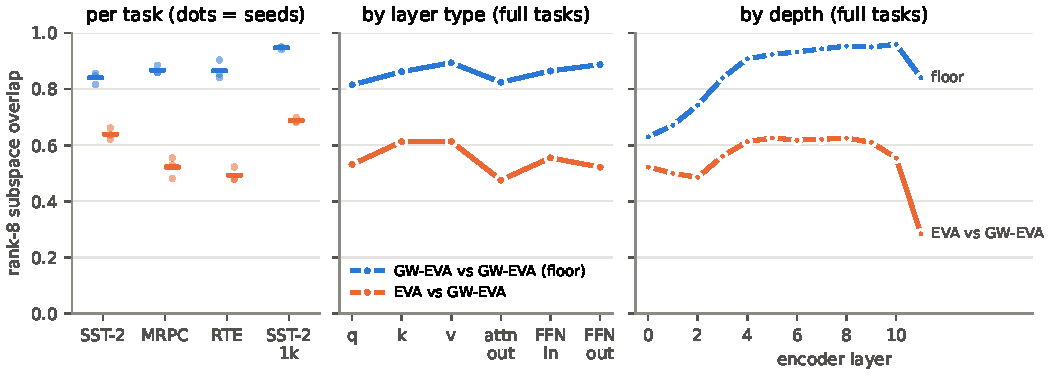
\includegraphics[width=0.84\textwidth]{figures/h1_overlap.pdf}
\caption{H1: overlap of GW-EVA with EVA on the same calibration sample (orange) against the GW-EVA noise floor (blue). Left: per task, dots are seeds. Middle and right: the three full-data tasks by layer type and by depth.}
\label{fig:h1}
\vspace{0.8em}
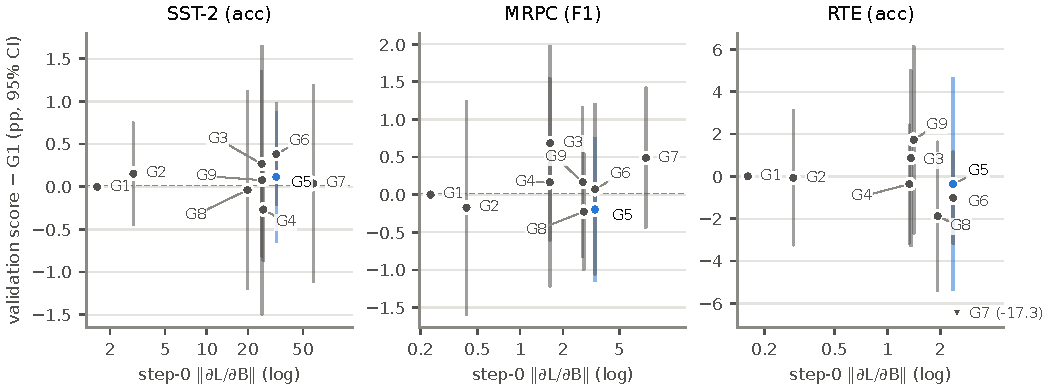
\includegraphics[width=0.84\textwidth]{figures/step0_vs_accuracy.pdf}
\caption{Step-0 $\norm{\partial L/\partial B}$ (log scale) against the accuracy difference to LoRA (G1), with 95\% intervals, per group and task. G5 (GW-EVA) is highlighted.}
\label{fig:step0}
\end{figure*}


\textbf{H1 is supported: GW-EVA picks a different subspace.} For each task and seed we sketch EVA (centred activation covariance) and GW-EVA ($\Sg$, uncentred) on the same 1,024 training examples, using the classification-head checkpoint of the shared runs, and compare their top-8 subspaces in all 72 layers. The noise floor compares GW-EVA estimated on two disjoint 1,024-example samples of the same task (Table~\ref{tab:h1}).

\begin{table}[t]
\centering
\small
\setlength{\tabcolsep}{2.5pt}
\begin{tabular}{@{}lccc@{}}
\toprule
Task & EVA vs GW & Floor & Difference \\
\midrule
SST-2 & 0.640 & 0.840 & $-0.201$ [$-0.224$, $-0.178$] \\
MRPC & 0.522 & 0.868 & $-0.346$ [$-0.439$, $-0.252$] \\
RTE & 0.493 & 0.866 & $-0.373$ [$-0.396$, $-0.350$] \\
Low-res.$^{\ddagger}$ & 0.688 & 0.947 & $-0.259$ [$-0.295$, $-0.223$] \\
\bottomrule
\end{tabular}
\caption{H1: top-8 subspace overlap of EVA and GW-EVA on the same sample, and the floor (GW-EVA on two disjoint samples), 3 seeds per task. Difference = overlap $-$ floor, paired by seed, 95\% CI. $^{\ddagger}$Both floor samples come from full SST-2 outside the 1k subset.}
\label{tab:h1}
\end{table}



The gap is significant on every task, and only 7 of 864 layer-seed pairs reach their floor. It is spread over all layer types and depths (Figure~\ref{fig:h1}). The attention output projection differs most (0.48 on the full tasks, against 0.61 for $k$ and $v$), as it does in H4. Over depth, the gap is smallest in layers 0--2, where the floor itself is only 0.63--0.74 because GW-EVA's own estimate is noisy there, and largest in the last layer (0.28 against a floor of 0.84). The mean principal angle between the two subspaces is 31--46$^\circ$. Per token, $\norm{g}^2$ is only weakly correlated with $\norm{x}^2$ (Pearson 0.10--0.19), so the gradient weighting is not a rescaled activation norm. The two halves of H1 thus come apart: the correlation with the input norm is weak, yet the weighting moves the subspace a lot.

\textbf{H2 is not supported.} GW-EVA's step-0 gradient is larger, as designed: 1.46$\times$, 2.27$\times$ and 2.00$\times$ EVA's on SST-2, MRPC and RTE, as means of same-seed ratios. But its accuracy is never significantly different, and all four mean differences are negative (Table~\ref{tab:paired}). H2's early-training claim fails too. At equal learning rates, G5 and G3 have the same training loss in steps 1--50 on every task. On SST-2, G5's loss is slightly higher afterwards ($+0.018$ in steps 51--200 and $+0.021$ in steps 201--500, both significant).

\subsection{Larger Gradients, Faster Start, Same Finish}
\label{sec:step0}


The step-0 gradient on $B$ grows 7--37$\times$ from LoRA to the data-aware initialisations, while accuracy stays within a one-point band (Figure~\ref{fig:step0}). The same-seed ratios in Table~\ref{tab:ratios} decompose this growth. The magnitude-only ratio G2/G1 matches the $\sqrt{3}$ predicted in Section~\ref{sec:identity} to within 6\%, which confirms the identity. EVA's directions then add another 4--8$\times$ at equal row norm, and GW-EVA a further 1.5--2.3$\times$. Yet G2, which changes only the norm, matches G1 in accuracy, and G3 and G5, which change the direction, match it as well.

\begin{table}[t]
\centering
\small
\setlength{\tabcolsep}{3pt}
\begin{tabular}{@{}lccc@{}}
\toprule
Task & G2/G1 (pred.\ 1.73) & G3/G2 & G5/G3 \\
\midrule
SST-2 & 1.83 (1.82--1.85) & 8.41 (6.54--10.64) & 1.46 (0.95--2.10) \\
MRPC & 1.78 (1.62--1.87) & 4.19 (3.08--7.17) & 2.27 (1.11--3.96) \\
RTE & 1.80 (1.66--1.92) & 4.48 (3.02--5.63) & 2.00 (0.84--3.13) \\
\bottomrule
\end{tabular}
\caption{Same-seed ratios of the step-0 gradient norm, mean (range). G2/G1 isolates magnitude, G3/G2 EVA's directions at equal norm, G5/G3 GW-EVA over EVA.}
\label{tab:ratios}
\end{table}

The gradient does buy a faster start. On MRPC, where all groups share lr $2\times10^{-4}$, EVA, GW-EVA and LoRA-GA have a significantly lower training loss than LoRA throughout the first 500 steps (Table~\ref{tab:loss}), but their final F1 is not significantly different. G2's loss differs from G1's by at most 0.004. A plausible reason why the gradient scale does not persist is Adam's per-coordinate normalisation, which removes most of the effect of the gradient's scale on the update size after the first few steps. We have not tested this directly.

\begin{table}[t]
\centering
\small
\setlength{\tabcolsep}{2.5pt}
\begin{tabular}{@{}lcccc@{}}
\toprule
Steps & 1--50 & 51--200 & 201--500 & Final F1 $-$ G1 \\
\midrule
G3 & $-0.015^{*}$ & $-0.054^{*}$ & $-0.038^{*}$ & $+0.68$ [$-0.60$, $+1.97$] \\
G5 & $-0.014^{*}$ & $-0.056^{*}$ & $-0.034^{*}$ & $-0.20$ [$-1.14$, $+0.75$] \\
G7 & $-0.024^{*}$ & $-0.054^{*}$ & $-0.039^{*}$ & $+0.49$ [$-0.44$, $+1.41$] \\
\bottomrule
\end{tabular}
\caption{MRPC, lr $2\times10^{-4}$: paired difference in mean training loss over each step window, group $-$ G1, for G3 (EVA), G5 (GW-EVA) and G7 (LoRA-GA).}
\label{tab:loss}
\end{table}

\subsection{Low Resource: the Gap Is the Learning Rate}

Under the shared rule, which reuses the full-SST-2 learning rate, every spectral initialisation trails LoRA by 1.6--3.1 points (Table~\ref{tab:paired}, last column). We reran the low-resource setting on one GPU outside the shared protocol to find out why (Table~\ref{tab:lowres}, Figure~\ref{fig:lowres}).

\begin{table}[t]
\centering
\small
\setlength{\tabcolsep}{3pt}
\begin{tabular}{@{}lccc@{}}
\toprule
Run & lr 2e-4 & lr 5e-4 & lr 1e-3 \\
\midrule
G1 LoRA & 91.44$\pm$0.22 & 91.44$\pm$0.28 & 91.47$\pm$0.66 \\
G3 EVA ($\rho=2$) & 90.87$\pm$0.55 & 90.55$\pm$0.54 & 89.50$\pm$1.16 \\
G3 EVA ($\rho=1$) & -- & -- & 89.08$\pm$0.42 \\
G8 EVA-generic & 90.41$\pm$1.15 & 90.28$\pm$0.69 & 89.89$\pm$0.52 \\
\bottomrule
\end{tabular}
\caption{Low-resource SST-2, 5 seeds, all on L40S. $\rho=1$ removes EVA's rank redistribution (uniform $r=8$).}
\label{tab:lowres}
\end{table}

\begin{figure}[t]
\centering
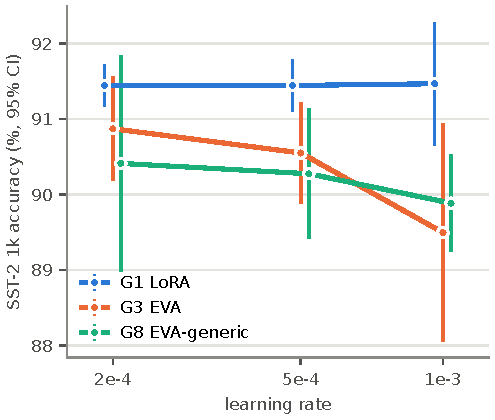
\includegraphics[width=0.85\columnwidth]{figures/lowres_lr.pdf}
\caption{Low-resource SST-2 accuracy against learning rate on one GPU (mean and 95\% interval over 5 seeds). LoRA is flat; EVA recovers at lower learning rates.}
\label{fig:lowres}
\end{figure}

\begin{figure*}[t]
\centering
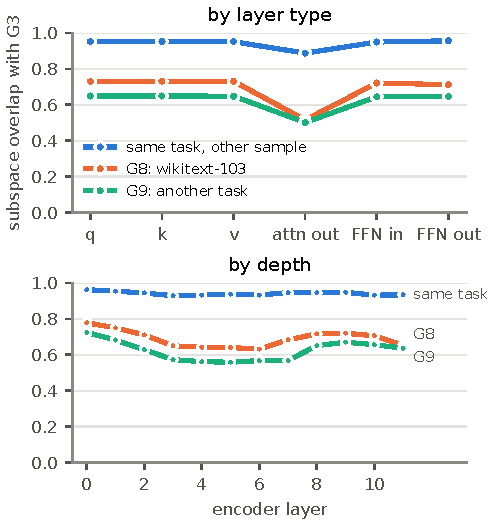
\includegraphics[width=0.78\textwidth]{figures/h4_layers.pdf}
\caption{H4: subspace overlap with same-task EVA for a disjoint same-task sample, G8 and G9, by layer type and by depth.}
\label{fig:h4}
\vspace{0.8em}
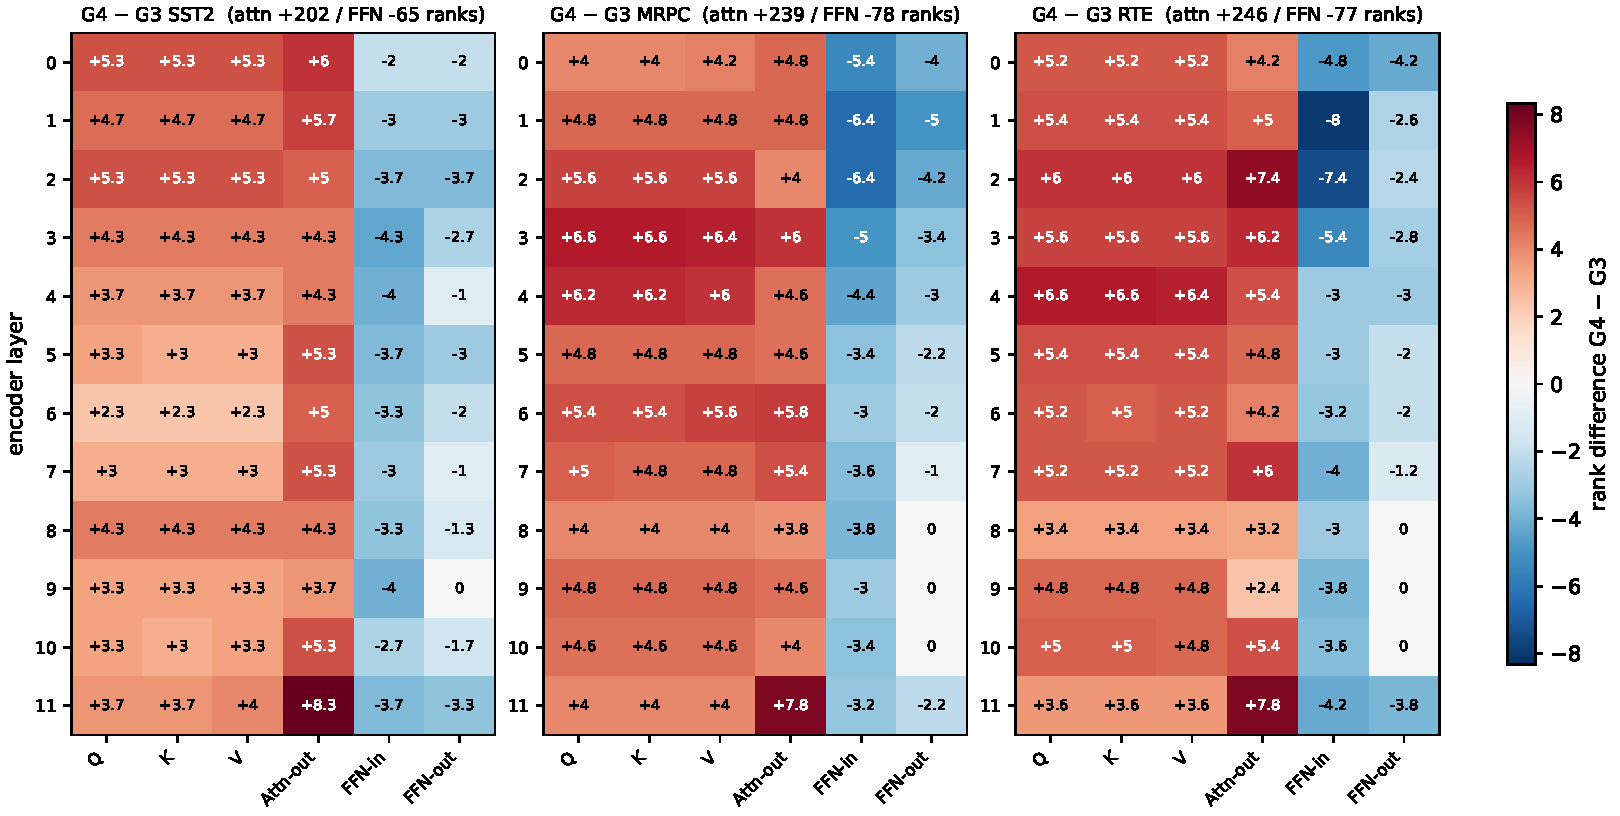
\includegraphics[width=0.8\textwidth]{figures/g34_rank_heatmap_diff.pdf}
\caption{H3: per-layer rank difference G4 $-$ G3 (red: G4 gives the layer more ranks), mean over main-stage seeds. Titles give the net change in attention and FFN ranks.}
\label{fig:ranks}
\end{figure*}

LoRA is insensitive to the learning rate, but EVA is not, and the shared rule gave EVA its worst setting. With both at $2\times10^{-4}$, G3 $-$ G1 $=-0.57$ [$-1.45$, $+0.30$], not significant. Removing EVA's rank redistribution changes nothing: $\rho=1$ vs $\rho=2$ gives $-0.41$ [$-2.32$, $+1.50$]. At lr $10^{-3}$ the loss curves show what goes wrong. EVA and GW-EVA start level with LoRA, then fit the training set more slowly in steps 51--200 ($+0.09$ and $+0.15$ over LoRA, both significant). This is an optimisation problem, not overfitting.

\subsection{Where the Calibration Data Comes From (H4)}

To separate real differences from sampling noise, the noise floor for H4 compares G3 with EVA computed on a disjoint 1,024-example sample of the same task (Table~\ref{tab:h4}). G9's MRPC and RTE columns compare the same pair of subspaces (EVA on MRPC vs EVA on RTE), so G9 gives two independent pairs, not three.

\begin{table}[t]
\centering
\small
\setlength{\tabcolsep}{4pt}
\begin{tabular}{@{}lccc@{}}
\toprule
Compared with G3 & SST-2 & MRPC & RTE \\
\midrule
Same task, disjoint sample (floor) & 0.919 & 0.951 & 0.951 \\
G8: wikitext-103, G3's layout & 0.642 & 0.716 & 0.694 \\
G9: another task & 0.493 & 0.662 & 0.662 \\
Random orthonormal, same ranks & 0.010 & 0.010 & 0.010 \\
\bottomrule
\end{tabular}
\caption{H4: overlap with same-task, same-seed EVA (G3).}
\label{tab:h4}
\end{table}


The calibration source moves 30--50\% of the subspace, far beyond the noise floor. The movement is uneven across layers (Figure~\ref{fig:h4}). By layer type, the attention output projection moves most (floor 0.89; G8 0.52; G9 0.50, against 0.65--0.73 for the other layer types). By depth, layers 3--7 move most. By input format, G8, which keeps G3's token layout and swaps only the words, overlaps more than G9, which changes both task and format. Most of that gap is on SST-2, where G9's calibration switches from single sentences to sentence pairs, so part of what looks like task content may be input format.

GW-EVA moves the subspace about as far from EVA's (0.49--0.69, Table~\ref{tab:h1}) as these calibration-source changes do. Accuracy does not follow. Neither G8 nor G9 is ever significantly different from LoRA on full data. Against G3, the only significant difference is G8 on MRPC ($-0.91$ [$-1.54$, $-0.28$]), which rests on G8's small variance and would not survive a multiplicity correction. \textbf{H4 is half supported:} EVA's subspace is task-specific, but at rank 8 the specificity does not matter for accuracy.

\subsection{Rank Allocation (H3)}

\textbf{H3 is not supported.} Allocating by parameter cost changes nothing on full data, for either direction: G4 $-$ G3 and G6 $-$ G5 are all non-significant (Table~\ref{tab:paired}). This holds although the allocation itself changes a lot (Figure~\ref{fig:ranks}). Because an attention rank costs 1,536 parameters and an FFN rank 3,840, G4 moves 202--246 ranks into the attention projections and 65--78 ranks out of the FFN layers. Mean ranks go from 8.8 to 13.6--13.7 for $q$, $k$ and $v$, and from 4.7 to 2.4 for the FFN output layer. G4 also spends the whole budget, while G3 stays 4.5--6.0\% under it, so G4 trains about 5\% more parameters and is still no better.


The one significant difference, G6 $-$ G5 $=+1.53$ in low resource, compares G6 at lr $5\times10^{-4}$ with G5 at lr $10^{-3}$. Given the low-resource results above, it most likely reflects the learning rate. Uniform ranks ($\rho=1$) also match EVA's redistribution in low resource.

\subsection{Robustness: RTE Collapse and GPU Effects}

\textbf{RTE collapse.} RTE is the least stable task. G7 (LoRA-GA) averages 56.68 on RTE: one seed predicts a single class for all 277 validation examples, and two are near chance. On SST-2 and MRPC it matches the other groups. Plain LoRA also collapses, on 1 of 10 seeds at its tuned lr $5\times10^{-4}$ and on none at $2\times10^{-4}$. At equal lr $2\times10^{-4}$ over 10 seeds, EVA beats LoRA on RTE: G3 $-$ G1 $=+2.13$ [$+0.97$, $+3.29$]. At LoRA's own tuned lr the difference is not significant ($+2.92$ [$-1.83$, $+7.68$], driven by the collapsed seed). EVA's gain on RTE is therefore one of robustness: it reaches good accuracy at a learning rate where LoRA is still slow, while LoRA reaches the same accuracy at a higher learning rate at the cost of occasional collapse.

\textbf{GPU effects.} We reran G3 with identical code, library versions and seeds on L40S instead of A40. Single low-resource seeds move by up to 2.5 points; the first training-step loss already differs, from bf16 numerics in the head warm-up. G3's MRPC mean drops by 1.08 [$-2.43$, $+0.27$]. With 15 MRPC seeds, EVA's apparent edge over LoRA is $+0.50$ [$+0.08$, $+0.92$] when G3's first five seeds come from A40, and shrinks to $+0.14$ [$-0.24$, $+0.51$] when all seeds run on L40S. Comparisons that decide a conclusion must therefore use one GPU.

%=====================================================================
\section{Discussion and Limitations}

The gradient identity holds, so GW-EVA does what it was designed to do: it maximises the expected step-0 gradient, and its gain over EVA is measurable. The quantity it optimises turns out to be the wrong target. Four results point the same way: the magnitude control (G2) shows that a larger gradient alone does nothing; the early-loss curves show that a faster start does not survive to the end of training; the low-resource controls show that EVA's apparent deficit is a learning-rate artefact; and the calibration-source controls and the H1 diagnostic show that the subspace can move by a third to a half, through other calibration data or through gradient weighting, without changing accuracy. At rank 8 on RoBERTa-base, the final accuracy is largely insensitive to which directions $A$ starts from. Table~\ref{tab:verdicts} summarises the verdicts.

\begin{table}[t]
\centering
\small
\begin{tabular}{@{}p{0.26\columnwidth}p{0.16\columnwidth}p{0.46\columnwidth}@{}}
\toprule
Hypothesis & Verdict & Evidence \\
\midrule
H1: $\Sg$'s subspace differs from EVA's & Supported & Overlap 0.49--0.69 vs floor 0.84--0.95, significant on all four settings \\
H2: GW-EVA beats EVA & Not supported & Larger step-0 gradient (1.5--2.3$\times$), no lower early loss, no higher accuracy \\
H3: allocation by parameter cost matters & Not supported & G4 $-$ G3, G6 $-$ G5 non-significant on full data despite large rank shifts \\
H4: subspace is task-specific and this matters & Half supported & Subspace moves 30--50\% with the calibration source; accuracy does not change \\
\bottomrule
\end{tabular}
\caption{Hypothesis verdicts.}
\label{tab:verdicts}
\end{table}

\textbf{Limitations.}
(1)~\emph{What H1 separates.} H1 compares centred EVA with uncentred $\Sg$, so the gap mixes the gradient weighting with centring. It uses top-8 subspaces rather than G5's allocated ranks, and its floor is GW-EVA against itself; the EVA--EVA floor (0.92--0.95) comes from the H4 script.
(2)~\emph{Mechanism.} The Adam explanation in the step-0 analysis is a hypothesis; training with SGD, or logging update norms, would test it.
(3)~\emph{Scope.} One encoder model, rank 8 and three GLUE tasks. Larger models, generative tasks or lower ranks, where the adapter's capacity binds, may behave differently.
(4)~\emph{Statistics.} Three to five seeds per cell for most groups, and no multiplicity correction; borderline single results such as G8 $-$ G3 on MRPC should be read with care.
(5)~\emph{Heterogeneous hardware and software.} G3/G4 ran on A40, G9 on a laptop GPU, and G5/G6 did not record their GPU. G5/G6 also use their own data loader, so their batch order is not paired with G1--G4. G7 uses older library versions and keeps weight decay 0.01 in the head warm-up. Our same-GPU reruns cover the comparisons that change conclusions, but not all comparisons.
(6)~\emph{Learning-rate coverage.} G5/G6 have no low-resource learning-rate controls and only three low-resource seeds, so we cannot say whether GW-EVA recovers at a lower learning rate the way EVA does.
(7)~\emph{Parameter count.} Rank-count allocation leaves G3, G8 and G9 3.8--6.4\% under budget, and G5 between 3.6\% under and 2.4\% over. This is reported, not corrected; for EVA it works against EVA, not for it.

%=====================================================================
\section{Conclusion}

Removing EVA's independence assumption gives an exact step-0 objective, a new initialisation (GW-EVA) and a unifying view of EVA and LoRA-GA. Under a carefully controlled, seed-paired comparison, GW-EVA does what the theory says: it maximises the initial gradient signal, with a subspace that differs from EVA's well beyond sampling noise (overlap 0.49--0.69 against a floor of 0.84--0.95). Neither it nor any other data-aware initialisation improves the final accuracy of RoBERTa-base with rank-8 LoRA. The commonly cited benefits of such initialisations, a larger initial gradient and faster early fitting, are real but transient. The few apparent accuracy gains come from the learning rate, from seed collapse, or from pairing runs across GPUs.

\section*{Contributions}

\begin{center}
\small
\begin{tabular}{@{}p{0.36\columnwidth}p{0.58\columnwidth}@{}}
\toprule
Member (branch) & Contribution \\
\midrule
{[Name]} (\texttt{yxh}) & G1/G2, magnitude control and theory check, extra seeds, same-GPU and learning-rate controls, H4 noise floor and per-layer analysis, cross-group summary and results page, report outline \\
Yin Chenyu (\texttt{yinchenyu\_g3g4}) & Shared data split and training pipeline, G3 EVA reproduction, G4 parameter-cost allocation, subspace-overlap metric, report writing \\
{[Name]} (\texttt{hanyanze}) & GW-EVA derivation and implementation, G5/G6, H1 subspace diagnosis \\
{[Name]} (\texttt{liyouran}) & G7 LoRA-GA \\
{[Name]} (\texttt{eddy\_G8}) & G8 EVA-generic, layout-preserving generic calibration, G8 overlap \\
{[Name]} (\texttt{zjz\_g9}) & G9 EVA-cross, H4 overlap analysis \\
\bottomrule
\end{tabular}
\end{center}

\bibliography{refs}

\end{document}
